\section{Deadlock Physics}\label{sec:physics}
% Budget 3.5 pages. Figs 2, 3, 4. Order (D9b): lone trap, noise as collective escape, pair standoff, arches.
\subsection{The Lone-Agent Trap at the Door Edges}\label{sec:lone}
\begin{figure}[t]
\centering
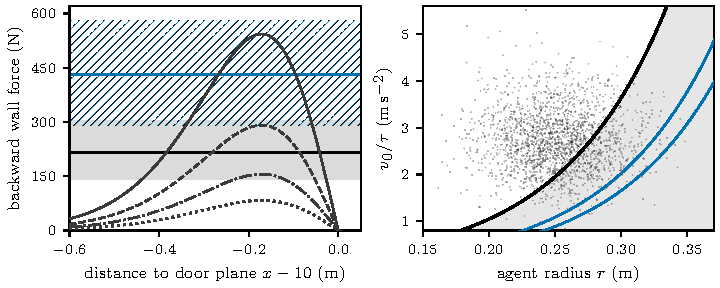
\includegraphics[width=\textwidth]{../figures/fig2_lone_trap.pdf}
\caption{Left: backward wall force on a lone agent on the door axis ($w=0.8$\,m) against distance to the door plane for $r=0.20$, 0.25, 0.30, 0.35\,m (dotted, dash-dotted, dashed, solid), and the rest-drive median and 5--95\% band for C1 (black) and C3 RVO2 (blue). Right: stuck-alone margin over $(r,v_0/\tau)$ from $-150$\,N (passes alone) to $+150$\,N (held alone), spawned agents as points, and margin-zero lines for C1 (black) and C3 RVO2 at $\tau=0.6$ and 0.4\,s (blue).}
\label{fig:lone-trap}
\end{figure}
%
On an agent at rest on the door axis, the lateral components of the two door-edge forces of Eq.~\eqref{eq:wall} cancel and their axial components push it back. The largest backward wall force along the axis, $g_{\max}(r)$, grows steeply with the radius $r$: \GmaxTwenty, \GmaxTwentyFive\ and \GmaxThirtyFive\,N at $r=0.20$, $0.25$ and $0.35$\,m (Fig.~\ref{fig:lone-trap}, left). Against it stands the drive at rest, $m v_{\rm eff}/\tau$. At the terminal rest state the blocker's Weidmann factor is at least \TermWeidMin\ (all \TermN\ deadlocks; Sect.~\ref{sec:model}). We therefore set $v_{\rm eff}=v_0$, and the agent is held alone if and only if
\begin{equation}\label{eq:stuck}
g_{\max}(r)>\frac{m\,v_0}{\tau}.
\end{equation}
The difference of the two sides is the stuck-alone margin. The C1 drive (median \DriveCOneMedian\,N, 5--95\%: \DriveCOneLo--\DriveCOneHi\,N) is comparable to $g_{\max}$ at the mean radius, so \EOneBStuckAloneFrac\ of the \StuckAloneN\ spawned agents are stuck alone; adding ORCA's rest drive (median \DriveORCAMedian\,N) lowers it to \StuckAloneFracCThree\ (Fig.~\ref{fig:lone-trap}, right). Fig.~\ref{fig:hero} (top) draws the energy along the blocker's axial coordinate with the other agents pinned.

At the rest state the criterion is a consistency check: a positive margin is necessary for a lone blocker to stay at rest. In the keystone test we removed every agent except the blocker, the agent nearest the door, from each of the \CriterionN\ deadlocks of both modes and restarted it. The \CriterionPosN\ blockers with positive margin all stayed held; \FixAfiveNearZeroN\ of the \CriterionN\ margins lie within $\pm10$\,N of zero. Of the \CriterionNegMargin\ blockers with negative margin, \CriterionNegTwoAgent\ belong to two-agent pair standoffs at the jamb faces (Sect.~\ref{sec:pair}) and the seventh to such a pair with two more agents away from the door. Each held blocker rests on the axis, stiffer sideways than along it (median Hessian eigenvalues \FixAfiveLatStiffMed\ and \FixAfiveAxStiffMed\,N/m).

Removing the blocker sorts corrected-forward deadlocks into keystone outcomes. In \KeystoneBLone\ the others leave (lone keystone), in \KeystoneBSecondTrap\ another agent takes the blocker's place and is held (second trap), and in \KeystoneBCollective\ the others stay as a group standoff (published-reproduction mode: \KeystoneALone, \KeystoneASecondTrap\ and \KeystoneACollective). The second trap is itself stuck alone in \SecondTrapHeld\ of \SecondTrapN\ cases, so most deadlocks are short stacks of stuck-alone agents. Whole runs rarely complete: \EOneBCompletionK\ of \EOneBCompletionN\ (corrected-forward) and \EOneACompletionK\ of \EOneACompletionN\ (published-reproduction).

The trap is set by the door width and the jamb wall law (Fig.~\ref{fig:width}; \EsevenN\ runs per setting). With the default walls, completion rises from \EsevenWSevenK\ of \EsevenN\ at $w=0.7$\,m and \EsevenWEightK\ at $0.8$\,m to \EsevenWTenK\ at $1.0$\,m. A logistic fit puts the critical width, where half the runs complete, at \EsevenWcrit\,m [\EsevenWcritLo, \EsevenWcritHi]. It lies between the width that holds the median spawned agent alone, \FixAeightWcMed\,m, and the width at which no agent of a run would be stuck alone, \FixAeightWfiftyPred\,m, because stuck-alone agents are often pushed through. At $w=0.8$\,m, shortening the range of every wall to $B_w=0.04$\,m lifts completion to \EsevenBallK\ of \EsevenN\ (\EsevenBallTwoK\ at $0.02$\,m), and shortening it on the jambs alone, to $B_{w,\rm edge}=0.04$\,m, to \EsevenBjambK\ ($p=\EsevenJambVsDefaultP$ against the default). The trap is therefore local to the door edges: shortening the other walls as well makes no detectable difference. Rounding the jamb corners or replacing the exit by a line goal leaves it in place (\EsevenRoundK, \EsevenLineK\ and \EsevenLineRoundK\ of \EsevenN). The short-range law also changes the type of the remaining deadlocks: pair or group standoffs make up \EsevenDefaultCollective\ of \EsevenDefaultClassified\ under the default walls and \EsevenBjambCollective\ of \EsevenBjambClassified\ with $B_{w,\rm edge}$ ($p=\EsevenCollectiveP$), \EsevenBallCollective\ of \EsevenBallClassified\ with all walls at $0.04$\,m and \EsevenBallTwoCollective\ of \EsevenBallTwoClassified\ at $0.02$\,m. It removes the lone traps (\EsevenBallLone\ remains with all walls at $0.04$\,m) and leaves the pair standoffs of Sect.~\ref{sec:pair}.

The order of arrival explains why the blocker is stuck alone. Agents that can pass alone leave first: the stuck-alone fraction is \ChainStuckEarlyMin--\ChainStuckFirstDecile\ over the first eight deciles of arrivals and \ChainStuckLastDecile\ in the last. The final blocker is among the last three arrivals in \ChainBlockerLastThree\ of \ChainBlockerN\ deadlocks. Stuck-alone agents push one another through: with no agent that could pass alone left, \ChainNoPassableExited\ of \ChainNoPassableN\ stuck-alone arrivals exit. The number of others active when a stuck-alone agent reaches the door predicts whether it exits (area under the ROC curve \EOneBAUCOthers\ [\EOneBAUCOthersLo, \EOneBAUCOthersHi]); the rule `exits if at least three others are active' classifies \EOneBRuleAcc\ of these agents correctly, against an all-exit baseline of \EOneBAllExitBaseline. The deadlock forms when the push behind the last stuck-alone agent runs out.

\begin{figure}[t]
\centering
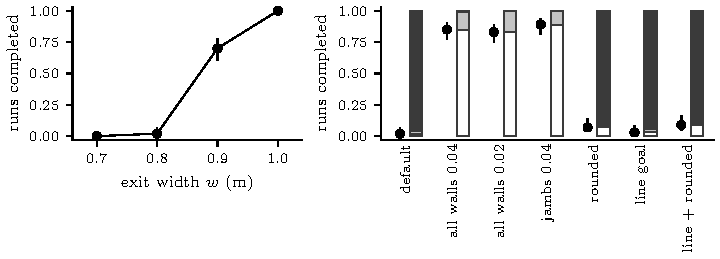
\includegraphics[width=\textwidth]{../figures/fig3_width_walls.pdf}
\caption{Fraction of C1 runs completed (point, Wilson 95\% interval) against exit width with the default walls (left), and at $w=0.8$\,m for each wall-law variant, labelled with its range $B_w$ in metres (right). Bars give the outcomes of all runs of a setting: completed (white), pair or group standoff (light grey), stack of stuck-alone agents (dark grey).}
\label{fig:width}
\end{figure}

\subsection{Noise as Collective Activated Escape}\label{sec:escape}
\begin{figure}[t]
\centering
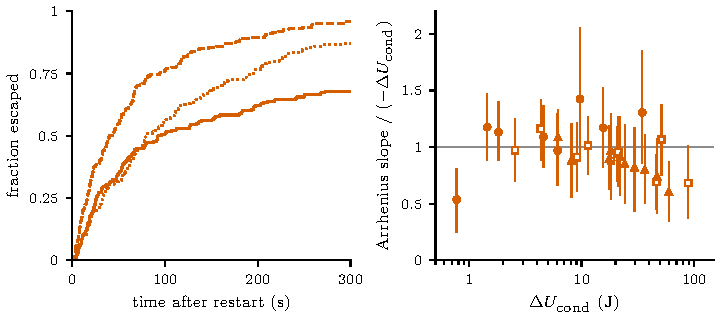
\includegraphics[width=\textwidth]{../figures/fig4_escape.pdf}
\caption{Left: Kaplan--Meier fraction of snapshots whose blocker has escaped against time at $\Delta U_{\rm cond}/k_BT_{\rm eff}=2.5$; right: escape rate over the fitted attempt rate against $\Delta U_{\rm cond}/k_BT_{\rm eff}$ for every snapshot, condition and noise level, with the predicted slope $-1$. Conditions, all in vermilion: full (solid, filled circles), pinned (dashed, open squares), alone (dotted, filled triangles).}
\label{fig:escape}
\end{figure}
%
We tested activated escape from the lone trap on \EfourN\ corrected-forward snapshots with at least two residual agents, spread over the full barrier (\FixAthreeEfourUsed\ of \FixAthreeEfourQual\ qualifying; \FixAthreeGateFailed\ of \FixAthreeGateTotal\ library barriers not accepted), in the three barrier conditions of Sect.~\ref{sec:signatures}. Eq.~\eqref{eq:teff} with the blocker's $\tau$ set the per-step noise so that $\Delta U/k_BT_{\rm eff}=1.5$, 2.5 and 3.5, with \EfourRestarts\ restarts per level, censored at 300\,s (900\,s at 3.5; \FixAthreeEfourCensFullPct\% of full-condition runs censored). Another agent's earlier exit does not end the run (\FixAthreeOtherExitFull\ of \FixAthreeOtherExitFullRuns\ full-condition runs). The full, pinned and alone conditions gave \EfourEventsFull, \EfourEventsFrozen\ and \EfourEventsAlone\ escapes.

The three predictions of activated escape hold with the exceptions below (Fig.~\ref{fig:escape}). The fitted slope of $\ln\lambda$ against $1/k_BT_{\rm eff}$ over $-\Delta U$ of the same condition has median \EfourRatioFull\ (full), \EfourRatioFrozen\ (pinned) and \EfourRatioAlone\ (alone), and its confidence interval covers 1 in \EfourCoverFull\ of \EfourFitsFull, \EfourCoverFrozen\ of \EfourFitsFrozen\ and \EfourCoverAlone\ of \EfourFitsAlone\ fits; the exceptions are \EfourNonCoverA\ (one full condition) and \EfourNonCoverB, \EfourNonCoverC\ (pinned and alone, one snapshot). Pooled with a free intercept per snapshot and condition, the rates fall on a line of slope $\FixAthreeCollapseSlope$ [$\FixAthreeCollapseSlopeLo$, $\FixAthreeCollapseSlopeHi$] against $\Delta U/k_BT_{\rm eff}$, shallower than the predicted $-1$. The pooled Weibull shape of the escape times, \EfourWeib\ [\EfourWeibLo, \EfourWeibHi], exceeds the exponential value 1. A lag fits better: with no escape before \FixAthreeLag\,s the shape is \FixAthreeShapeAtLag\ [\FixAthreeShapeAtLagLo, \FixAthreeShapeAtLagHi], and counted from 2\,s it is \FixAthreeShapeTwo\ [\FixAthreeShapeTwoLo, \FixAthreeShapeTwoHi], except in the pinned condition (\FixAthreeShapeFrozenTen\ [\FixAthreeShapeFrozenTenLo, \FixAthreeShapeFrozenTenHi] from 10\,s). The median attempt rates are \EfourNuFull\,s$^{-1}$ (full) and \EfourNuAlone\,s$^{-1}$ (alone), a median \FixAthreeNuRatioAll\ of the Langer prefactor from the Hessians at minimum and saddle (below it in \FixAthreeNuRatioBelow\ of \FixAthreeNuRatioN\ fits). The escape is collective: the full barrier lies below the alone barrier in \EfourSaddleBelow\ of \EfourSaddleN\ snapshots (median ratio \FixAthreeSaddleRatioFitted\ over the \FixAthreeSaddleFittedN\ fitted). The neighbours carry a median share \FixAthreeNeighbourDispMed\ of the displacement from minimum to saddle; the blocker carries the unstable mode at the saddle (participation ratio \FixAthreePRMed).

Two snapshots are left out of the fits. In one, a marginally stable deadlock, the full barrier of \EfourSkippedDU\,J lies below the 0.1\,J noise-setting floor. In the other (\EfourSeedOneSeventyResid\ residual agents, accepted full barrier \EfourSeedOneSeventyDU\,J) none of the \EfourSeedOneSeventyRestarts\ restarts at any noise level escapes within 300\,s (\EfourSeedOneSeventyEvents\ events). The computed path is not the route the dynamics takes; we cannot explain why.

For whole runs, half complete at noise amplitude $\sigma_{50}=\EfiveSigmaFifty$ [\FixAsixSigFiftyClLo, \FixAsixSigFiftyClHi]\,m/s in the corrected-forward mode and $\EfiveASigmaFifty$ [\FixAsixSigFiftyPubClLo, \FixAsixSigFiftyPubClHi]\,m/s in the published-reproduction mode (\EfiveN\ runs per level; logit fits; intervals resample seeds, whose outcomes correlate across levels). The conference estimate, \EfiveConfSigmaFifty\,m/s from 25 runs per level~\cite{gang2026}, lies at the upper edge of both.

\subsection{The Pair Standoff at the Jamb Faces}\label{sec:pair}
In the second type every agent would pass the door if it were alone. Two agents stand before the jamb faces, one on each side of the door axis, \PairAxisMin--\PairAxisMax\,m from it, with a surface gap of \PairGapMin--\PairGapMax\,m; neither touches the other or a wall. Each is driven toward the door and pushed sideways toward the axis, and the pair repulsion holds off the two lateral pushes. We built a library of \PairN\ such snapshots from independent corrected-forward runs with $B_{w,\rm edge}=0.04$\,m. Fig.~\ref{fig:hero} (bottom) shows one, with the wall force drawn for $B_w=0.08$\,m above the axis and $0.04$\,m below it. We call the member below the axis in that view the lower member; the handedness probe counts which member exits first.

With the densities frozen the rest field is $-\nabla U$ of Eq.~\eqref{eq:U} (largest residual \PairResidMax\,N), so the Hessian of $U$ in the four member coordinates sets its stability. It is positive definite in \PairStrictMin\ of \PairN\ snapshots: every standoff is a strict local minimum. The softest eigenvalue, $\mu_1=\PairLamOneMin$--\PairLamOneMax\,N/m (median \PairLamOneMed), belongs in all \PairSoftCommon\ to the common lateral shift of both members; the opposed lateral mode is next, stiffer by a factor of \PairLamRatioMin--\PairLamRatioMax. As Proposition~\ref{prop:rest} predicts, the standoff survives every small displacement: it stays held in every unperturbed C1 restart and in all \PairPerturbN\ replays perturbed by $10^{-9}$\,m, and a common lateral shift of both members frees \PairDeltaOneMmFreed\ of \PairN\ at 1\,mm and \PairDeltaOneCmFreed\ at 1\,cm. A shift of 3\,cm carries \PairDeltaThreeCmFreed\ of \PairN\ out of the basin.

A lateral bias $b$ tilts every desired direction the same way and so loads the soft mode. The strict minimum survives small tilts and is lost at a threshold $b_f$, which we located for each snapshot and sign by overdamped relaxation under bias, bisecting in $b$. For the sign with the lower threshold, $b_f=\PairBstarMin$--\PairBstarMax\ (median \PairBstarMed). The signs differ because the members stand at unequal distances from the axis (rank correlation of the difference with this asymmetry \PairAsymCorr). \pending{after the continuation run: whether $\mu_1$ reaches zero at $b_f$ as a saddle-node fold} The static prediction, freed if $|b|>b_f$ and held otherwise, agrees with the 120\,s quench in \PairFoldAgree\ of \PairFoldN\ (snapshot, $b$) cases for the eight bias values $|b|\le0.1$ (Wilson lower bound \PairFoldLo). All \PairFoldFN\ disagreements are quenches that escape at a bias at most \PairFoldMissGap\% below the snapshot's static threshold; the members' inertia carries them over. The freed fraction rises from \PairBiasOneFreed\ of \PairN\ at $b=0.01$ to \PairBiasTenFreed\ at $b=0.1$ (Fig.~\ref{fig:pair}, left), and the member on the favoured side exits first in all \PairHandAll\ freed runs.

The minimum is shallow. On \PairBarN\ snapshots spread over $\mu_1$, the string method of Sect.~\ref{sec:signatures} gives pair barriers of \PairBarMin--\PairBarMax\,J (median \PairBarMed\,J), well below the lone-trap barrier (median \LoneBarMed\,J over the \LoneBarN\ accepted library barriers; 3\,J and above in the time-step test of Sect.~\ref{sec:att-lone}), and $\mu_1$ does not predict them (rank correlation $\PairBarSpearman$). Noise of $\sigma=0.01$\,m/s frees \PairNoiseLowFreed\ of \PairNoiseLowN\ runs. $\Delta U/k_BT_{\rm eff}$ is below 1 at every noise level for \FixAthreePairBelowOne\ of the \FixAthreePairN\ snapshots, so the Arrhenius test of Sect.~\ref{sec:escape} has no lever arm. The escape times are not exponential (pooled Weibull shape \PairWeibLow\ at $\sigma=0.01$ and \PairWeibHigh\ at $0.05$\,m/s): once off the shallow minimum, the pair needs a few seconds of deterministic run-out to clear the door.

\subsection{No Persistent Contact Arches}\label{sec:arches}
A granular clog is an arch of grains in contact, held by normal forces and static friction~\cite{zuriguel2014}. The SFM has no static friction: the tangential contact force of Eq.~\eqref{eq:sfm} is proportional to the relative sliding velocity and vanishes at rest, so a contact arch stands only while its normal forces balance. We drove the bottleneck hard (corrected-forward C1, $w=0.8$\,m, 100 agents with mean desired speed \ArchVZero\,m/s, \ArchN\ runs of up to 600\,s) and searched every 0.1\,s for a chain of agents in mutual contact touching both jambs. They form in \ArchRunsWithArch\ of \ArchN\ runs (\ArchEpisodes\ episodes, \ArchEpisodesThree\ with three or more agents, up to \ArchSizeMax) and carry up to \ArchPeakForce\,kN of body compression, but break within \ArchMaxLife\,s (95\% within \ArchPNinetyFive\,s). None lasts 10\,s (\ArchPersistent\ of \ArchN\ runs, upper Wilson bound \ArchPersistentHi), and every run completes (\ArchComplete\ of \ArchN), at the tested time step $\Delta t=0.01$\,s \pending{after the resolution run: unchanged at $\Delta t=0.0025$\,s and at the default drive}. The model's persistent deadlocks are the contact-free rest states of Sects.~\ref{sec:lone} and~\ref{sec:pair}, soft-core analogues of one- and two-grain arches, held by repulsion of range $B_w$ rather than by contact and friction.
